%part2.tex
\part{\LaTeX{}图形宏包套件}

\section{加入 EPS 图像文件}\label{sec:inserteps}

关于~\pai{graphics}~和~\pai{graphicx}~宏包的最好的参考资料是
~\textsl{Graphics guide}\cite{grfguide}~和~\textsl{\LaTeX{} Graphics
	Compannion}\cite{Michel-1}。其它的~\LaTeX{}~参考资料中对~\textsf{graphicx}~
包只是零星的介绍。~\cite{Helmut}~中对~\textsf{graphics}~和~\textsf{graphicx}~
都作了介绍,~\cite{Leslie}~中只介绍了~\textsf{graphics}包,而~\cite{Michel}~
中两者均未提及。

\subsection{includegraphics 命令}\label{ssec:includegraphics}

{\large\hspace{1cm}
	\color{morelight}{\shadowbox{\textcolor{blue}{\texttt{%
					\bs includegraphics[\CJKfamily{kai}选项]\{文件\}}}}}}

这里的{\CJKfamily{kai}选项}在表~\ref{tab:opt},
\ref{tab:cropopt}, \ref{tab:boolopt}~中列出。
因为~\cmd{includegraphics}~不会结束
当前段落,所以它能够在文本中放置图形如
~\includegraphics[width=12pt]{recycle}~和~

\includegraphics[width=12pt]{illusion}。下面的命令将以~\texttt{file.eps}~
的自然大小插入到~\LaTeX{}~文档中:

\begin{Verbatim}[xleftmargin=1cm]
\documentclass{article}
\usepackage{graphicx}
\begin{document}
\includegraphics{file.eps}
\end{document}
\end{Verbatim}

\begin{table}
	\newcommand{\tbltt}[1]{\textcolor{cyan}{\texttt{#1}}}
	\renewcommand{\arraystretch}{1.2}
	\centering
	\topcaption{\texttt{includegraphics Options}}\label{tab:opt}
	
	\begin{tabular}{>{\columncolor{morelight}}l|>{\CJKfamily{kai}}m{11cm}|}
		
		\cline{2-2}
		\tbltt{height} & 图形的高度(可为任何~\TeX{}~度量单位)。 \\
		\cline{2-2}
		\tbltt{totalheight} & 图形的全部高度,可为任何~\TeX{}~度量单位(
		\textsl{6/95~增加})。 \\
		\cline{2-2}
		\tbltt{width} & 图形的宽度(可为任何~\TeX{}~度量单位)。\\
		\cline{2-2}
		\tbltt{scale} & 图形的缩放因子,设定~\texttt{scale=2}~会使
		插入的图形的大小为其自然大小的两倍。\\
		\cline{2-2}
		\tbltt{angle} & 设定旋转的角度,以度为单位,顺时钟方向为正。\\
		\cline{2-2}
		\tbltt{origin} & \texttt{origin}~指定图形绕那一点旋转,缺省
		是图形的参考点(\textsl{12/95~增加})。初始点有可能与
		第~\ref{sec:rotatebox}节的~\cmd{rotatebox}~命令中的一样。
		比如~\texttt{origin=c}~将使图形绕它的中心旋转。 \\
		\cline{2-2}
		\tbltt{bb} &  设定~BoundingBox~的值。
		~\texttt{bb=10 20 100 200}~设定~BoundingBox~的左下角在
		~\texttt{(10,20)},右上角在~\texttt{(100,200)}。因为
		~\cmd{includegraphics}~会自动从~EPS~文件中读入~BoundingBox~行
		所给的值,所以一般不使用~\texttt{bb}~这个选项。但它在~EPS~文件
		中的~BoundingBox~丢失或出错时还是很有用的。\\
		\cline{2-2}
	\end{tabular}
\end{table}

\begin{table}
	\newcommand{\tbltt}[1]{\textcolor{cyan}{\texttt{#1}}}
	\renewcommand{\arraystretch}{1.2}
	\centering
	\topcaption{\texttt{includegraphics Cropping Options}}\label{tab:cropopt}
	
	\begin{tabular}{>{\columncolor{morelight}}l|>{\CJKfamily{kai}}m{10cm}|}
		
		\cline{2-2}
		\tbltt{viewpoint} & 指定图形可以被看到的部分。如同~BoundingBox~一样,
		这是一个由四个数字,左下角和右上角的坐标所确定的区域。
		这里的坐标是相对于~BoundingBox~的左下角的(
		\textsl{6/95~增加})。
		
		例如,如果图形的~BoundingBox~的值是~\texttt{50
			50 410 302},~\texttt{viewpoint=50 50 122 122}~
		将显示以图形的左下角为左下角的一英寸大小的区域。
		而~\texttt{viewpoint=338 230 410 302}~则会显示以图形的
		右上角为右上角的一英寸大小的区域。
		
		必须使用~\texttt{clip}~选项(见表~\ref{tab:boolopt})
		来阻止显示视图以外的图形部分 。 \\
		\cline{2-2}
		\tbltt{trim} &   指定图形可以被看到的部分的另一选项。所给出的四个数字
		分别代表了从左、下、右、上被截去的值。正数代表从此方向
		截去的大小,而负数则代表从此方向加上的大小。 \\
		\cline{2-2}
	\end{tabular}
\end{table}

\begin{table}
	\newcommand{\tbltt}[1]{\textcolor{cyan}{\texttt{#1}}}
	\renewcommand{\arraystretch}{1.2}
	\centering
	\topcaption{\texttt{includegraphics Boolean Options}}\label{tab:boolopt}
	
	\begin{tabular}{>{\columncolor{morelight}}l|>{\CJKfamily{kai}}m{10cm}|}
		
		\cline{2-2}
		\tbltt{noclip} & (缺省选项)显示整个的图形,即使有些部分在视图之外。 \\
		\cline{2-2}
		\tbltt{clip} & 当使用~\texttt{clip}~时,将不显示图形在视图之外的部分。 \\
		\cline{2-2}
		\tbltt{draft} & 当使用~\texttt{draft}~选项时,将只显示图形的~BoundingBox~
		和文件名,这使得显示和打印文档的速度加快。如果使用
		~\texttt{draft}~宏包选项,\verb+\usepackage[draft]{graphicx}+
		会导致文档中的所有图形都被以草稿(\texttt{draft})方式插入。\\
		\cline{2-2}
		\tbltt{final} & (缺省选项,除非使用\verb+\usepackage[draft]{graphicx}+)
		~\texttt{final}~选项使得图形被显示,经常用来覆盖~
		\verb+\usepackage[draft]{graphicx}+ \\
		\cline{2-2}
		\tbltt{keepaspectratio} & 在没有设定~\texttt{keepaspectratio}~选项时,
		给定图形的高度(全部高度)和宽度会导致图形被不对称缩
		放来满足所设定的高和宽。在设定~\texttt{keepaspectratio}~
		选项后,给定图形的高度(全部高度)和宽度时,图形会
		保持原有的宽高比例,尽可能使得图形满足所设定的高和宽,
		但是图形不会超出其中任一个。 \\
		\cline{2-2}
	\end{tabular}
\end{table}

如果加入的图形文件没有指明扩展名,那么~\cmd{includegraphics}~会根据
~\cmd{DeclareGraphicsExtensions}~的扩展名列表自动为它加上扩展名(见第~
\ref{sec:deextension}~节)。由于缺省的扩展名列表不包括空的扩展名,
~\cmd{includegraphics\{file\}}~不会读入~\texttt{file}。除非空的扩展名
已被加到扩展名列表中。

\noindent{\CJKfamily{hei}命令} \marginpar{\CJKfamily{kai}\bfseries 指定宽度}
\begin{Verbatim}[xleftmargin=1cm]
\includegraphics[width=3in]{file.eps}
\end{Verbatim}

将~\texttt{file.eps}~插入文档并且它的宽度被缩放到~3~英寸,高度也会
按相应的比例缩放。如果用~\cmd{textwidth}~或~\cmd{em}~等的函数来
指定宽度,而不是用像~3~英寸这样的固定尺寸,将会使你的~\LaTeX{}~文
档更具通用性。例如:
\begin{Verbatim}[xleftmargin=1cm]
\includegraphics[width=\textwidth]{graphics.eps}
\end{Verbatim}
将所插入图形缩放到和文本行的宽度一样宽。而下面的命令
\begin{Verbatim}[xleftmargin=1cm]
\includegraphics[width=0.80\textwidth]{graphics.eps}
\end{Verbatim}
使得插入图形的宽度为文本行宽的~$80\%$。当与~\pai{calc}~宏包配合使用
时,下面的命令可令图形的宽度比文本行宽少~2~英寸:
\begin{Verbatim}[xleftmargin=1cm]
\includegraphics[width=\textwidth-2.0in]{graphics.eps}
\end{Verbatim}

\hbox to \textwidth{%
	\hfill({\CJKfamily{kai}需要~\textsf{graphicx} \textsl{12/95}~或以后的
		版本。})}

下面是一些使用~\cmd{includegraphics}~命令来插入图形的
例子。这里为方便起见,定义~\ci{HR}~如下:
\begin{Verbatim}[xleftmargin=1cm]
\newcommand{\HR}{\rule{1em}{0.4pt}}
\end{Verbatim}

\ifpdf\else %因为使用pdflatex不支持clip.所以省去。
\noindent 在下面的几个例子中可以看到使用~\texttt{bb,clip,viewport}~
和~\texttt{trim}~的效果。

\hspace{-1cm}\begin{minipage}[c]{.5\textwidth}
	左\HR%
	\fbox{%
		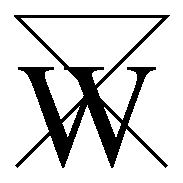
\includegraphics[bb=120 120 150 200]{w.eps}}%
	\HR 右
	\qquad
	左\HR%
	\fbox{%
		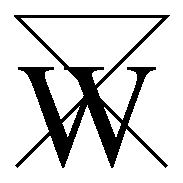
\includegraphics[bb=120 120 150 200,clip]{w.eps}}%
	\HR 右
\end{minipage}%
\begin{minipage}[c]{.5\textwidth}
	\begin{Verbatim}[frame=lines,label=\colorbox{green}{\small 例一},labelposition=topline,]
	左\HR\fbox{%
	\includegraphics
	[bb=120 120 150 200]%
	{w.eps}}%
	\HR 右
	\qquad
	左\HR\fbox{%
	\includegraphics
	[bb=120 120 150 200,clip]%
	{w.eps}}%
	\HR 右
	\end{Verbatim}
\end{minipage}

\hspace{-1.5cm}\begin{minipage}[c]{.65\textwidth}
	左\HR\fbox{%
		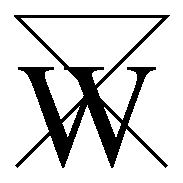
\includegraphics[viewport=20 20 50 100,clip]{w}}%
	\HR 右
	\qquad
	左\HR\fbox{%
		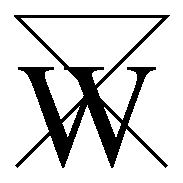
\includegraphics[trim=5 5 10 10,clip]{w}}%
	\HR 右
\end{minipage}%
\hspace{-1cm}\begin{minipage}[c]{.5\textwidth}
	\begin{Verbatim}[frame=lines,label=\colorbox{green}{\small 例二},labelposition=topline]
	左\HR\fbox{%
	\includegraphics
	[viewport=20 20 50 100,clip]%
	{w.eps}}%
	\HR 右
	\qquad
	左\HR\fbox{%
	\includegraphics
	[trim=5 5 10 10,clip]%
	{w.eps}}
	\HR 右
	\end{Verbatim}
	\par\vspace{0pt}
\end{minipage}
\fi

\noindent 在下面的几个例子中,可以比较以下使用~\texttt{scale,width,height,angle}~
以及~\texttt{keepaspectratio}~选项及其不同的顺序所得到的不同效果。

\begin{minipage}[t]{.45\textwidth}
	\vspace{0pt}
	左\HR\fbox{%
		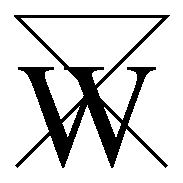
\includegraphics[scale=.5]{w}}\HR 右
\end{minipage}%
\hspace{-.5cm}\begin{minipage}[t]{.5\textwidth}
	\vspace{0pt}
	\begin{Verbatim}[frame=lines,label=\colorbox{green}{\small 例一},labelposition=topline]
	左\HR\fbox{%
	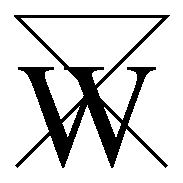
\includegraphics
	[scale=.5]{w.eps}%
	\HR 右
	\end{Verbatim}
\end{minipage}

\begin{minipage}[c]{.45\textwidth}
	左\HR\fbox{%
		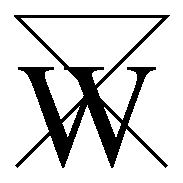
\includegraphics[width=10mm]{w}}\HR 右
\end{minipage}%
\hspace{-.5cm}\begin{minipage}[c]{.5\textwidth}
	\begin{Verbatim}[frame=lines,label=\colorbox{green}{\small 例二},labelposition=topline]
	左\HR\fbox{%
	\includegraphics%
	[width=10mm]{w.eps}%
	\HR 右
	\end{Verbatim}
\end{minipage}

\begin{minipage}[c]{.45\textwidth}
	左\HR\fbox{%
		\includegraphics[height=20mm,width=30mm]%
		{w}}\HR 右
\end{minipage}%
\hspace{-.5cm}\begin{minipage}[c]{.5\textwidth}
	\begin{Verbatim}[frame=lines,label=\colorbox{green}{\small 例三},labelposition=topline]
	左\HR\fbox{%
	\includegraphics
	[height=20mm,width=30mm]%
	{w.eps}}\HR 右
	\end{Verbatim}
\end{minipage}

\begin{minipage}[c]{.45\textwidth}
	左\HR\fbox{%
		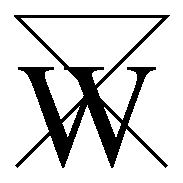
\includegraphics[height=20mm,width=30mm,%
		keepaspectratio]{w}}\HR 右
\end{minipage}%
\hspace{-.5cm}\begin{minipage}[c]{.5\textwidth}
	\begin{Verbatim}[frame=lines,label=\colorbox{green}{\small 例四},labelposition=topline]
	左\HR\fbox{%
	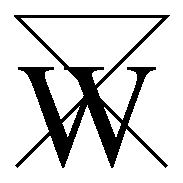
\includegraphics
	[height=20mm,width=30mm,%
	keepaspectratio]{w.eps}}%
	\HR 右
	\end{Verbatim}
\end{minipage}

\begin{minipage}[c]{.45\textwidth}
	左\HR\fbox{%
		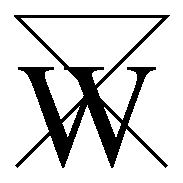
\includegraphics[angle=-45]{w}}\HR 右
\end{minipage}%
\hspace{-.5cm}\begin{minipage}[c]{.5\textwidth}
	\begin{Verbatim}[frame=lines,label=\colorbox{green}{\small 例五},labelposition=topline]
	左\HR\fbox{%
	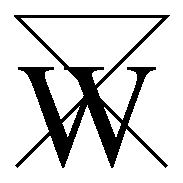
\includegraphics
	[angle=-45]{w.eps}}%
	\HR 右
	\end{Verbatim}
\end{minipage}

\begin{minipage}[c]{.45\textwidth}
	左\HR\fbox{%
		\includegraphics[angle=-45,width=30mm]%
		{w}}\HR 右
\end{minipage}%
\hspace{-.5cm}\begin{minipage}[c]{.5\textwidth}
	\begin{Verbatim}[frame=lines,label=\colorbox{green}{\small 例六},labelposition=topline]
	左\HR\fbox{%
	\includegraphics
	[angle=-45,width=30mm]%
	{w.eps}}\HR 右
	\end{Verbatim}
\end{minipage}

\hspace{-1cm}\begin{minipage}[c]{.45\textwidth}
	左\HR\fbox{%
		\includegraphics[width=30mm,angle=-45]%
		{w}}\HR 右
\end{minipage}%
\begin{minipage}[c]{.5\textwidth}
	\begin{Verbatim}[frame=lines,label=\colorbox{green}{\small 例七},labelposition=topline]
	左\HR\fbox{%
	\includegraphics
	[width=30mm,angle=-45]%
	{w.eps}}\HR 右
	\end{Verbatim}
\end{minipage}

\begin{minipage}[c]{.45\textwidth}
	左\HR\fbox{%
		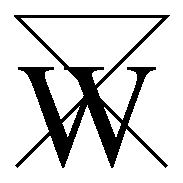
\includegraphics[angle=-60,totalheight=15mm]{w}}%
	\HR 右
\end{minipage}%
\hspace{-.5cm}\begin{minipage}[c]{.5\textwidth}
	\begin{Verbatim}[frame=lines,label=\colorbox{green}{\small 例八},labelposition=topline]
	左\HR\fbox{%
	\includegraphics
	[angle=-60,totalheight=15mm]%
	{w.eps}}%
	\HR 右
	\end{Verbatim}
\end{minipage}

\begin{minipage}[c]{.45\textwidth}
	左\HR\fbox{%
		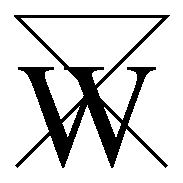
\includegraphics[angle=-60,totalheight=20mm,width=30mm]{w}}%
	\HR 右
\end{minipage}%
\hspace{-.5cm}\begin{minipage}[c]{.5\textwidth}
	\begin{Verbatim}[frame=lines,label=\colorbox{green}{\small 例九},labelposition=topline]
	左\HR\fbox{%
	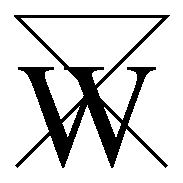
\includegraphics
	[angle=-60,totalheight=20mm,%
	width=30mm]{w.eps}}%
	\HR 右
	\end{Verbatim}
\end{minipage}

\begin{minipage}[c]{.45\textwidth}
	左\HR\fbox{%
		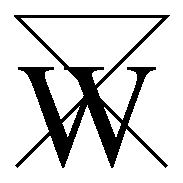
\includegraphics[angle=-60,totalheight=20mm,width=30mm,keepaspectratio]{w}}%
	\HR 右
\end{minipage}%
\hspace{-.5cm}\begin{minipage}[c]{.5\textwidth}
	\begin{Verbatim}[frame=lines,label=\colorbox{green}{\small 例十},labelposition=topline]
	左\HR\fbox{%
	\includegraphics
	[angle=-60,totalheight=20mm,%
	width=30mm,keepaspectratio]%
	{w.eps}}%
	\HR 右
	\end{Verbatim}
\end{minipage}

\section{旋转和缩放对象}\label{sec:scalerotate}

除了上一章介绍的~\cmd{includegraphics}~命令外,~\textsf{graphicx}~宏包还提供了
另外四个命令用来旋转和缩放任意的~\LaTeX{}~对象:{\CJKfamily{kai}文本,
	~EPS~图形等等。}

\begin{Verbatim}[xleftmargin=1cm, formatcom=\CJKfamily{kai}\color{blue}]
\scalebox{水平缩放因子}[垂直缩放因子]{对象}
\resizebox{宽度}{高度}{对象}
\resizebox*{宽度}{全部高度}{对象}
\rotatebox[选项]{角度}{对象}
\end{Verbatim}

因为~\textsf{graphicx}~包的~\cmd{includegraphics}~带有支持旋转和缩放的
~\texttt{angle}~和~\texttt{width}~等选项,所以本章介绍的这几个命令很少
在插图时使用。例如:
\begin{Verbatim}[xleftmargin=1cm]
\includegraphics[scale=2]{file.eps}
\includegraphics[width=4in]{file.eps}
\includegraphics[angle=45]{file.eps}
\end{Verbatim}
上述命令和下面的命令等到的结果是相同的。
\begin{Verbatim}[xleftmargin=1cm]
\scalebox{2}{\includegraphics{file.eps}}
\resizebox{4in}{!}{\includegraphics{file.eps}}
\rotatebox{45}{\includegraphics{file.eps}}
\end{Verbatim}

尽管结果相同,但在实际使用中最好还是用前一种方法,因为它能更迅速的
生成效率更高的~\PS。

\clearpage

\subsection{scalebox 命令}\label{ssec:scalebox}

{\large\hspace{1cm}
	\color{morelight}{\shadowbox{\textcolor{blue}{\texttt{%
					\bs scalebox\{\CJKfamily{kai}水平缩放因子\}[垂直缩放因子]\{对象\}}}}}}

\ci{scalebox}~命令对其作用的对象进行缩放,使缩放后的对象的宽度为原始
宽度与水平缩放因子之积,高度为原始高度与垂直缩放因子之积。如果垂直缩放
因子没有给出,那么将按照给定的水平缩放因子,保持原始宽高的比例进行缩放。
如果缩放因子为负值,则对对象进行反射。下面是几个例子:

\hspace{-1.5cm}\begin{minipage}[b]{.5\textwidth}
	\begin{center}
		\color{blue}{\CJKfamily{kai}
			\scalebox{2}{%
				这是放大的文字} \\
			这是正常的文字 \\
			\scalebox{.5}{%
				这是缩小的文字}}
	\end{center}
	\par\vspace{0pt}
\end{minipage}%
\begin{minipage}[b]{.5\textwidth}
	\begin{Verbatim}[formatcom=\color{VerbatimColor}\CJKfamily{kai}]
	\scalebox{2}{这是放大的文字} \\
	这是正常的文字  \\
	\scalebox{.5}{这是缩小的文字}
	\end{Verbatim}
	\par\vspace{0pt}
\end{minipage}

\hspace{-1.5cm}\begin{minipage}[b]{.5\textwidth}
	\color{blue}{\CJKfamily{kai}
		\framebox{\scalebox{2}{%
				\parbox{.5in}{放大 \\ 和 \\ 缩小}}}
		\framebox{\scalebox{2}[1.5]{%
				\parbox{.5in}{放大 \\ 和 \\ 缩小}}}}
	\par\vspace{0pt}
\end{minipage}%
\begin{minipage}[b]{.5\textwidth}
	\begin{Verbatim}[formatcom=\color{VerbatimColor}\CJKfamily{kai}]
	\framebox{\scalebox{2}{%
	\parbox{.5in}{放大 \\ 和 \\ 缩小}}}
	\framebox{\scalebox{2}[1.5]{%
	\parbox{.5in}{放大 \\ 和 \\ 缩小}}}
	\end{Verbatim}
	\par\vspace{0pt}
\end{minipage}

\hspace{-1.5cm}\begin{minipage}[b]{.5\textwidth}
	\begin{center}
		\color{blue}{\texttt{%
				China? \scalebox{-1}[1]{China?} \\
				China? \scalebox{1}[-1]{China?} \\
				China? \scalebox{-1}[-1]{China?} \\
				China? \scalebox{-1}{China?}}}
	\end{center}
	\par\vspace{0pt}
\end{minipage}%
\begin{minipage}[b]{.5\textwidth}
	\begin{Verbatim}
	China? \scalebox{-1}[1]{China?} \\
	China? \scalebox{1}[-1]{China?} \\
	China? \scalebox{-1}[-1]{China?} \\
	China? \scalebox{-1}{China?}}
	\end{Verbatim}
	\par\vspace{0pt}
\end{minipage}

\subsection{resizebox 命令}\label{ssec:resizebox}

{\large\hspace{1cm}{\color{morelight}{\shadowbox{\textcolor{blue}{\texttt{%
						\bs resizebox\{\CJKfamily{kai}宽度\}\{高度\}\{对象\}}}}}}}

{\large\hspace{1cm}{\color{morelight}{\shadowbox{\textcolor{blue}{\texttt{%
						\bs resizebox$\ast$\{\CJKfamily{kai}宽度\}\{全部高度\}\{对象\}}}}}}}

\ci{resizebox}~命令将对象的大小改变为给定值。如果{\CJKfamily{kai}宽度}
或{\CJKfamily{kai}高度}中的任一项用~!~给出,则其代表的选项的长度在被改变
大小时会保持原有的宽高比例不变。例如:
~\verb+\resizebox{2in}{!}{argument}+~将对象的宽度改变为~2~英寸。

标准的~\LaTeXe{}~长度~\cmd{height}, \cmd{width}, \cmd{totalheight},
\cmd{depth}~可用来表示对象的原始尺寸。因此,
~\verb+\resizebox{2in}{\height}{argument}+~使得对象的宽度改变为~2~英寸
但保持原有高度不变。 除了第二个参数表示对象的全部高度以外,
~\ci{reseizebox$\ast$}~与~\cmd{resizebox}~是相同的。下面是几个例子:

\hspace{-1.5cm}\begin{minipage}[b]{.5\textwidth}
	\begin{center}
		\color{blue}{\CJKfamily{kai}
			\framebox{\resizebox{5mm}{!}{%
					\parbox{14mm}{选项 \\ 角度 \\ 对象}}}
			\framebox{\resizebox{!}{10mm}{%
					\parbox{14mm}{选项 \\ 角度 \\ 对象}}}}
		\par\vspace{0pt}
	\end{center}
\end{minipage}%
\hspace{-1cm}\begin{minipage}[b]{.5\textwidth}
	\begin{Verbatim}[formatcom=\color{VerbatimColor}\CJKfamily{kai}]
	\framebox{\resizebox{5mm}{!}{%
	\parbox{14mm}{选项 \\ 角度 \\ 对象}}}
	\framebox{\resizebox{!}{10mm}{%
	\parbox{14mm}{选项 \\ 角度 \\ 对象}}}
	\end{Verbatim}
	\par\vspace{0pt}
\end{minipage}

\hspace{-2cm}\begin{minipage}[b]{.5\textwidth}
	\begin{center}
		\color{blue}{\CJKfamily{kai}
			\resizebox*{2cm}{3cm}{\LaTeX{}~图形} \\
			\resizebox*{2cm}{1cm}{\LaTeX{}~图形}}
		\par\vspace{0pt}
	\end{center}
\end{minipage}%
\begin{minipage}[b]{.5\textwidth}
	\begin{Verbatim}[formatcom=\color{VerbatimColor}\CJKfamily{kai}]
	\resizebox*{2cm}{3cm}{\LaTeX{}~图形} \\
	\resizebox*{2cm}{1cm}{\LaTeX{}~图形}
	\end{Verbatim}
	\par\vspace{0pt}
\end{minipage}

\subsection{rotatebox 命令}\label{ssec:rotatebox}

{\large\hspace{1cm}
	\color{morelight}{\shadowbox{\textcolor{blue}{\texttt{%
					\bs rotatebox[\CJKfamily{kai}选项]\{角度\}\{对象\}}}}}}

\ci{rotatebox}~将对象旋转一给定度数的角度,逆时针方向为正。缺省地,
对象绕它的参考点旋转。~\cmd{rotatebox}~命令中的~{\CJKfamily{kai}选项}
允许对象绕给定的点来旋转。

\begin{enumerate}
	\item 给定~\verb+[x=xdim,y=ydim]+,则对象旋转所绕的点相对于参考点的
	坐标为~\verb+(xdim,ydim)+。
	\item \texttt{origin}~选项指定~12~个特殊点其中之
	一(见图~\ref{fig:rotatepoint})。
	
	\texttt{origin}~点的水平位置由~\texttt{lcr}~(分别代表左、中、右)其中
	之一确定,垂直位置则由~\texttt{t,c,B,b}~(分别代表顶部、中部、基线、底部)
	中的一个来确定。例如:
	\begin{description}
		\item [\texttt{[rb]}] 右下角。
		\item [\texttt{[lt]}] 左上角。
		\item [\texttt{[cB]}] 图形基线的中点。
	\end{description}
	{\CJKfamily{hei}几点说明:}
	\begin{itemize}
		\item 标记字母的顺序并不重要,~\texttt{[br]}~就等于~\texttt{[rb]}。
		\item \texttt{c}~代表水平位置的中点还是垂直位置的中点靠和它一起的
		标记字母来决定。
		\item 如果只给出一个标记字母,那么另一个将被假设为~\texttt{c}。
		即~\texttt{[c]}~等于~\texttt{[cc]},~\texttt{[l]}~等于
		~\texttt{[lc]},~\texttt{[t]}~等于~\texttt{[ct]}~等等。
	\end{itemize}
\end{enumerate}

\begin{figure}
	\centering
	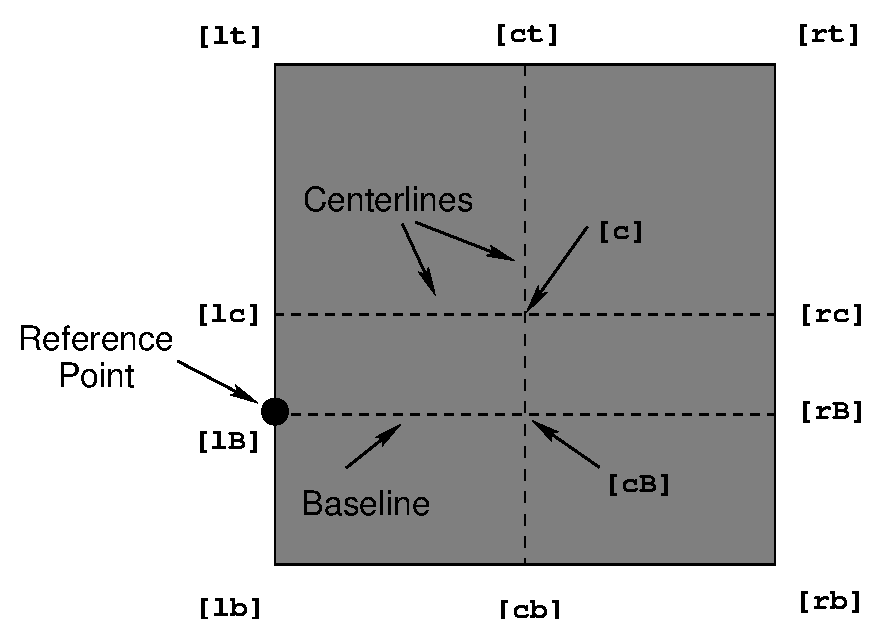
\includegraphics[width=.6\textwidth]{orig-point}
	\caption{Available Origin Point}\label{fig:rotatepoint}
\end{figure}

\noindent 下面是一个例子:

\hspace{-1.5cm}\begin{minipage}[b]{.5\textwidth}
	\begin{center}
		\setlength{\fboxsep}{0mm}
		\newcommand{\MyRot}[1]{%
			\fbox{\rotatebox{#1}{旋转~$#1^\circ$}}}
		\color{blue}{\CJKfamily{kai}
			\MyRot{0} \MyRot{45} \MyRot{90}
			\MyRot{135} \MyRot{180} \MyRot{225}}
	\end{center}
	\par\vspace{0pt}
\end{minipage}%
\begin{minipage}[b]{.5\textwidth}
	\begin{Verbatim}[formatcom=\color{VerbatimColor}\CJKfamily{kai}]
	\setlength{\fboxsep}{0mm}
	\newcommand{\MyRot}[1]{%
	\fbox{\rotatebox{#1}{旋转~$#1^\circ$}}}
	\MyRot{0} \MyRot{45} \MyRot{90}
	\MyRot{135} \MyRot{180} \MyRot{225}
	\end{Verbatim}
	\par\vspace{0pt}
\end{minipage}

\section{高级命令}\label{sec:adgraph}

本章描述了一些在下述情形下使用的~\LaTeXe{}~图形宏包套件的高级命令。

\begin{enumerate}
	\item 当使用没有扩展名的文件名时。如:
	\begin{Verbatim}[xleftmargin=1cm]
	\includegraphics{file}
	\end{Verbatim}
	\item 当使用压缩的~EPS~图形文件时。见第~\ref{sec:compresseps}~节。
	\item 当使用非~EPS~格式的图形文件时。见第~\ref{sec:noneps}~节。
\end{enumerate}

在这些情况下,~\LaTeX{}~如何处理由~\cmd{includegraphics}~所引入的
文件,就需要用~\ci{DeclareGraphicsRule}~和~\ci{DeclareGraphicsExtensions}~
命令来控制。

\begin{itemize}
	\item \cmd{DeclareGraphicsExtensions}~命令指定了在没有提供图形文件扩展名的
	情况下,~\LaTeX{}~将自动为其加上的扩展名列表(如~\texttt{.eps, .ps,
		.eps.gz}~等)。
	\item \cmd{DeclareGraphicsRule}~命令指定了对图形文件执行的命令。执行这一
	命令要求操作系统支持管道功能,比如~Unix~等操作系统,而~DOS~则不行。
	
	若将此命令指定为一解压缩命令,那么就可以使用压缩的~EPS~图形文件。
	若将此命令指定为一图形格式转换命令,那么就可以使用非~EPS~格式的图形文件。
\end{itemize}

\clearpage

\subsection{DeclareGraphicsExtensions 命令}\label{ssec:deextension}

\cmd{DeclareGraphicsExtensions}~命令告诉~\LaTeX{},若~\cmd{includegraphics}~命令
所引入的文件没有提供扩展名,将试图为其自动加上什么样的扩展名。为方便起见,
在选择图形驱动\realfootnote{指定一个图形驱动选项如
	~\texttt{\bs usepackage[dvips]\{graphics\}}~将会覆盖掉在~\texttt{graphics.cfg}~中
	设定的缺省驱动选项}时,就已经有一个相应的预设的扩展名集。举例来说,如果
选择~\texttt{dvips}~作为图形驱动,那么缺省地会使用下列图形文件扩展名(在
~\texttt{dvips}~中定义):
\begin{Verbatim}[xleftmargin=1cm]
\DeclareGraphicsExtensions{.eps,.ps,.eps.gz,.ps.gz,.eps.Z}
\end{Verbatim}
这时,\cmd{includegraphics\{file\}}让~\LaTeX{}~首先寻找~\texttt{file.eps},
其次~\texttt{file.ps},再其次~\texttt{file.eps.gz},直到找到一个文件。
相应地,你就可以在~\LaTeX{}~文件中用
\begin{Verbatim}[xleftmargin=1cm]
\includegrapincs{file}
\end{Verbatim}
取代
\begin{Verbatim}[xleftmargin=1cm]
\includegrapincs{file.eps}
\end{Verbatim}
这样做的好处是如果你以后决定压缩~\texttt{file.eps},你也无须更改~\LaTeX{}~文件。

\noindent{\CJKfamily{hei}说明:}\marginpar{\CJKfamily{kai}\bfseries无扩展名的
	\\ 文件}
\begin{Verbatim}[xleftmargin=1cm]
\includegrapincs{file}
\end{Verbatim}
不会试图寻找~\texttt{file},除非空的扩展名~\verb+{}+~已被加入到扩展名列表中。
例如:
\begin{Verbatim}[xleftmargin=1cm]
\DeclareGraphicsExtensions{.eps,.eps.gz,{}}
\end{Verbatim}
将试图在没找到~\texttt{file.eps}~和~\texttt{file.eps.gz}~的情况下
寻找~\texttt{file}。

不给出扩展名\marginpar{\CJKfamily{kai}\bfseries Pool Space \\ 问题}
而靠~\LaTeX~从
~\cmd{DeclareGraphicsExtensions}~的扩展名列表中选择正确的扩展名可能
加重~pool space~问题(见第~\ref{sec:poolspace}~节)。如果有
~pool space~问题的话,应当使扩展名列表中的扩展名数目尽可能小。如:
\begin{Verbatim}[xleftmargin=1cm]
\DeclareGraphicsExtensions{.eps,.eps.gz}
\end{Verbatim}

\clearpage

\subsection{DeclareGraphicsRule 命令}\label{ssec:derule}

\ci{DeclareGraphicsRule}~命令指定~\cmd{includegraphics}~如何按照文件的扩展名
来对图形文件进行操作。可以允许有多个~\cmd{DeclareGraphicsRule}~命令。

{\large\hspace{1cm}
	\color{morelight}{\shadowbox{\textcolor{blue}{\texttt{%
					\bs DeclareGraphicsRule\{ext\}\{type\}\{sizefile\}\{command\}}}}}}

\begin{table}
	\newcommand{\tbltt}[1]{\textcolor{cyan}{\texttt{#1}}}
	\renewcommand{\arraystretch}{1.2}
	\centering
	\topcaption{\texttt{DeclareGraphicsRule Arguments}}\label{tab:Declaregrule}
	
	\begin{tabular}{>{\columncolor{morelight}}l|>{\CJKfamily{kai}}m{10cm}|}
		\cline{2-2}
		\tbltt{ext} & 文件的扩展名。 \\
		\cline{2-2}
		\tbltt{type} & 扩展名所对应的图形格式。 \\
		\cline{2-2}
		\tbltt{sizefile} & 包含图形的~BoundingBox~的文件的扩展名。如果这一选项为空,
		那么须要在~\cmd{includegraphics}~命令中给定~\texttt{bb}~项
		的值。 \\
		\cline{2-2}
		\tbltt{command} & 作用于图形文件的命令,此项常为空。命令前必须有一个后向单引号
		(而不是常使用的前向单引号)。目前为止,只有~\texttt{dvips}~能
		够使用这样的命令。参见第~\ref{chap:noneps}~章用这样的命令
		来处理非~EPS~格式图形和压缩~EPS~图形的例子。\\
		\cline{2-2}
	\end{tabular}
\end{table}

例如:
\begin{Verbatim}[xleftmargin=1cm]
\DeclareGraphicsRule{.eps.gz}{eps}{.eps.bb}{`gunzip -c #1}
\end{Verbatim}
指定任何以~\texttt{.eps.gz}~为扩展名的文件为压缩~EPS~文件,该文件
的~BoundingBox~信息存放在扩展名为~\texttt{.eps.bb}~的文件中,并
用命令~\texttt{gunzip -c}~来解压缩(因为~\LaTeX{}~不能从压缩文件中
读取~BoundingBox~信息,所以~BoundingBox~行必须存放到一非压缩文件中)。

\cmd{DeclareGraphicsRule}~命令允许使用~$\ast$~代表任何未知扩展名,
例如:
\begin{Verbatim}[xleftmargin=1cm]
\DeclareGraphicsRule{*}{eps}{*}{}
\end{Verbatim}
会导致所有未知扩展名的文件都被认为是~EPS~文件,比方说~\texttt{file.EPS}~
就被当做~EPS~文件。

这里文件名里第一个句点 \marginpar{\CJKfamily{kai}\bfseries 文件名中的 \\ 句点}
以后的部分都被认为是文件的扩展名,这样做是为了能够
正确地识别压缩的~EPS~文件(扩展名为~\texttt{.eps.gz})等。为了避免
混淆,文件的基本名中不要使用句点。否则~\texttt{file.name.eps.gz}~会让
~\cmd{includegraphics}~寻找扩展名为~\texttt{.name.eps.gz}~所对应的规则,
由于这样的规则很有可能不存在,结果导致使用未知扩展名所对应的规则。
例外的情形是该文件的格式正好是缺省格式,如未知扩展名的文件
都被认为是~EPS~文件时,那么~\texttt{file.name.eps}~就能被正确地识别。

为方便起见,\marginpar{\CJKfamily{kai}\bfseries 预先定义的 \\ 命令}根据不同的图形驱动选项
\realfootnote{指定一个图形驱动选项如~\texttt{\bs usepackage[dvips]\{graphics\}}~
	将会覆盖掉在~\texttt{graphics.cfg}~中设定的缺省驱动选项}
预定义了不同的缺省图形规则。例如使用~\texttt{dvips}~图形驱动选项
时,缺省图形规则为:

\begin{Verbatim}[xleftmargin=1cm]
\DeclareGraphicsRule{.eps}{eps}{.eps}{}
\DeclareGraphicsRule{.ps}{eps}{.ps}{}
\DeclareGraphicsRule{.pz}{eps}{.bb}{`gunzip -c #1}
\DeclareGraphicsRule{.eps.Z}{eps}{.eps.bb}{`gunzip -c #1}
\DeclareGraphicsRule{.ps.Z}{eps}{.ps.bb}{`gunzip -c #1}
\DeclareGraphicsRule{.eps.gz}{eps}{.eps.bb}{`gunzip -c #1}
\DeclareGraphicsRule{.ps.gz}{eps}{.ps.bb}{`gunzip -c #1}
\DeclareGraphicsRule{.pcx}{bmp}{}{}
\DeclareGraphicsRule{.bmp}{bmp}{}{}
\DeclareGraphicsRule{.msp}{bmp}{}{}
\DeclareGraphicsRule{*}{eps}{*}{}
\end{Verbatim}

前面两个命令定义扩展名为~\texttt{.eps}~和~\texttt{.ps}~的文件为~EPS~文件,
它们后面的五个命令定义了压缩~EPS~文件的扩展名和解压命令,
接下来的三个命令定义了位图文件的扩展名(见第~\ref{sec:noneps}~节),
最后一个命令设定未知扩展名的文件为~EPS~文件。

\endinput

